% vim:ts=4:sw=4
%
% Copyright (c) 2008-2009 solvethis
% Copyright (c) 2010-2012 Casper Ti. Vector
% Public domain.
%
% 使用前请先仔细阅读 pkuthss 和 biblatex-caspervector 的文档,
% 特别是其中的 FAQ 部分和用红色强调的部分。
% 两者可在终端/命令提示符中用
%   texdoc pkuthss
%   texdoc biblatex-caspervector
% 调出。

% 在黑白打印时彩色链接可能变成浅灰色,此时可将“colorlinks”改为“nocolorlinks”。
\documentclass[UTF8, colorlinks, notocbibind]{pkuthss}

% 使用 biblatex 排版参考文献,并规定其格式。
\usepackage[backend = biber, style = sysu, utf8]{biblatex}
% 使得打字机粗体可以被使用。
\usepackage{lmodern}
% 产生 originauth.tex 里的 \square。
\usepackage{amssymb}
% 提供 Verbatim 环境和 \VerbatimInput 命令。
\usepackage{fancyvrb}
% 图像包
\usepackage{subcaption}
% --引入其他pdf文件--
\usepackage[cmex10]{amsmath}
\usepackage{algorithmic}
\usepackage{array}
\usepackage{pdfpages}

% 使被强调的内容为红色。
\newcommand{\myemph}[1]{\emph{\textcolor{red}{#1}}}

% pkuthss 文档模版的版本。
\newcommand{\docversion}{v1.4 rc1}

% 设定文档的基本信息。
\pkuthssinfo{
	cthesisname = {本科生毕业论文}, ethesisname = {Undergraduate Thesis},
	ctitle = {基于力与扭力信号\\对错误组装案例进行识别},
	% “\\”在设定 pdf 属性时会被自动过滤掉,于是得到的 pdf 属性中标题为
	%   The PKU dissertation document classpkuthss [版本号]
	% 此处指定其被替换为“: ”,以使之为
	%   The PKU dissertation document class: pkuthss [版本号]
	etitle = {%
		Early Failure Assembly CasesDetection \texorpdfstring{\\}%
		Based on Force/Torque Signal%
	},
	cauthor = {罗伟强},
	eauthor = {Waldron Luo},
	studentid = {10389321},
	date = {二〇一四年三月},
	school = {软件学院},
	cmajor = {软件工程}, emajor = {Software Engineering},
	direction = {嵌入式系统与软件},
	cmentor = {Dr. Juan Rojas}, ementor = {Dr. Juan Rojas},
    ckeywords = {力信号,支持向量机,基于梯度变化的分类法},
    ekeywords = {Force/Toruqe, Support Vector Machine, Relative-Change-Based-Hierachical-Taxonomy-System}
}
% 导入参考文献数据库(注意不要省略“.bib”)。
\addbibresource{mybib.bib}
\addbibresource{xbib.bib}

%\includeonly{chap/chap1, chap/chap2}

\begin{document}
	% 以下为正文之前的部分。
	\frontmatter

	% 自动生成标题页。
	\maketitle
	% --可以使用includepdf直接将转换好的附表或封面加入--
	%\includepdf[pages=1-2]{chap/cover.pdf}
	%\includepdf[pages=1-2]{chap/report.pdf}
	%\includepdf[pages=1-2]{chap/check.pdf}
	%\includepdf[pages=1-2]{chap/reply.pdf}
	%\includepdf[pages=1-2]{chap/statement.pdf}
	% 版权声明。
%	% vim:ts=4:sw=4
%
% Copyright (c) 2008-2009 solvethis
% Copyright (c) 2010-2012 Casper Ti. Vector
% All rights reserved.
%
% Redistribution and use in source and binary forms, with or without
% modification, are permitted provided that the following conditions are
% met:
%
% * Redistributions of source code must retain the above copyright notice,
%   this list of conditions and the following disclaimer.
% * Redistributions in binary form must reproduce the above copyright
%   notice, this list of conditions and the following disclaimer in the
%   documentation and/or other materials provided with the distribution.
% * Neither the name of Peking University nor the names of its contributors
%   may be used to endorse or promote products derived from this software
%   without specific prior written permission.
% 
% THIS SOFTWARE IS PROVIDED BY THE COPYRIGHT HOLDERS AND CONTRIBUTORS "AS
% IS" AND ANY EXPRESS OR IMPLIED WARRANTIES, INCLUDING, BUT NOT LIMITED TO,
% THE IMPLIED WARRANTIES OF MERCHANTABILITY AND FITNESS FOR A PARTICULAR
% PURPOSE ARE DISCLAIMED. IN NO EVENT SHALL THE COPYRIGHT HOLDER OR
% CONTRIBUTORS BE LIABLE FOR ANY DIRECT, INDIRECT, INCIDENTAL, SPECIAL,
% EXEMPLARY, OR CONSEQUENTIAL DAMAGES (INCLUDING, BUT NOT LIMITED TO,
% PROCUREMENT OF SUBSTITUTE GOODS OR SERVICES; LOSS OF USE, DATA, OR
% PROFITS; OR BUSINESS INTERRUPTION) HOWEVER CAUSED AND ON ANY THEORY OF
% LIABILITY, WHETHER IN CONTRACT, STRICT LIABILITY, OR TORT (INCLUDING
% NEGLIGENCE OR OTHERWISE) ARISING IN ANY WAY OUT OF THE USE OF THIS
% SOFTWARE, EVEN IF ADVISED OF THE POSSIBILITY OF SUCH DAMAGE.

\chapter*{版权声明}
{
	\zihao{3}\linespread{1.5}\selectfont

	任何收存和保管本论文各种版本的单位和个人,
	未经本论文作者同意,不得将本论文转借他人,
	亦不得随意复制、抄录、拍照或以任何方式传播。
	否则一旦引起有碍作者著作权之问题,将可能承担法律责任。
	\par
}


	% 中英文摘要。
	% vim:ts=4:sw=4
%
% Copyright (c) 2008-2009 solvethis
% Copyright (c) 2010-2012 Casper Ti. Vector
% Public domain.

\begin{cabstract}
    错误检测在现代工业进程以及机器人服务,特别是无规则环境的作业中,担任越来越重要的角色。我们主要研究了悬臂卡扣组装中的错误检测技术。它在工业应用以及个人机器人中有着重要的地位。

    \indent 我们希望根据卡扣组装过程的力信号特征,用小集合的特征向量来抽象组装过程,并且据此来训练支持向量机分类法,从而在组装任务的不同阶段精确地检测组装过程中发生的错误。在我们的实验中,我们通过抽象行为特征训练了一个线性支持向量机,从而进行卡扣组装的错误检测。这个方法在早/晚期的错误检测中非常有效。在早期错误检测中,抽象程度较低的行为特征集相对于高度抽象集表现得更好,这是因为在其局部时间内颗粒度更加精细的原因。在晚期错误检测中,高度抽象集表现得更好,因为对于全局的组装动作,高度抽象集更好地表示了组装动作。
    
\end{cabstract}

\begin{eabstract}

    Failure detection plays an increasingly important role in industrial processes and robots that serve in unstructured environments. This work studies failure detection on cantilever snap assemblies, which are critical to industrial use and growing in importance for personal use. 
    
    \indent Our aim is to study whether an SVM can use a small set of features abstracted as behavior representations from the assembly force signature to accurately detect failure at different stages of the task. In this work, a linear SVM was embedded with abstract behavioral features was used to classify failure detection in cantilever snap assembly problems. The approach was useful in detecting failure both during early and late stages of the task. For early stages, low-abstraction behaviors sets performed better due to their granularity and local temporal nature. For late stage analysis, high-abstraction behaviors performed better as they capture representative and global behaviors better.

\end{eabstract}


	% 自动生成目录。
	\tableofcontents

	% 以下为正文。
	\mainmatter

	% 绪言。
	% % vim:ts=4:sw=4
%
% Copyright (c) 2008-2009 solvethis
% Copyright (c) 2010-2012 Casper Ti. Vector
% Public domain.

\specialchap{Introduction}

Uncertain failure occurs during a assembly task to the severe detriment to the assembly parts and the robot hands. Failures should be detected as early as possible and actions should be taken. In our work, we used SVM to identify the failure cases and detect the failure early in the assembly process.
\indent In our previous work, we built the framework for snap assembly in varying geometric complexity, including the generalizable strategy and controllers\cite{2012JAR-Rojas-AutHetBotAsmbly} \cite{2012ICMA-Rojas-PivotApproach}, the state estimation\cite{2012IROS-Rojas-RCBHT}, the failure characterization\cite{2012Humanoids-Rojas-pRCBHT}. All our contribution are integrated in \cite{2013IJMA-Rojas-TwrdsSnapSensing}. \\
\indent The failure identification technique previously used was pRCBHT\cite{2013IJMA-Rojas-TwrdsSnapSensing}. pRCBHT is consist of RCBHT, which is a taxonomy used multi layer labels to sample the assembly process, and bayesian filter, which takes the labels as input and predict the result of the assembly with Markovian assumption. In this paper, rather than using the probabilistic methods, Support Vector Machine(SVM) is used instead. Compared to bayesian filter, SVM is an easier approach in implementing and more intuitive to the classification. In our case, SVM was used with Primitive labels, Motion Composites labels (MC), Low-level Behaviors labels which are increasingly abstracted. The more abstracted labels contains less information but more refining. On the contrary, the less abstracted labels contains more information embodying the abundant noise. \\
\indent SVM is one of the most widely used classification approach contemporarily. Compared to data-driven method using SVM\cite{masonfailure}, RCBHT is Rather than data-driven, the labels of RCBHT can be said as gradient-driven. The premise of data-driven methods is that the success cases would have similar curves of signals. Similar curves also had similar upwards and downwards, and so we tried RCBHT with SVM to classify the assembly cases. \\
\indent With LLB labels and MC labels of the whole process, failure cases can be identified. With the Approach state of Primitive labels, early failure detection is done in our approach. This is significant when failure detection is done early in assembly because cancellation and redoing can be called in time for prevention and cut the cost.\\
\indent Other approaches including \cite{rodriguez2011abort} and \cite{di2013bayesian}, signals were trainedwith Hidden Markov Model (HMM). Their methods are more general, but RCBHT was specially developed for the cantilever-snap assembly and increasingly abstracted layers will be more data-rich. \\
\indent Though our approach has a high accrucy in identify failure cases. ....There is two limits. The first one is that with RCBHT, this approach is not general for other force/torque signal analysis. The second one is that the failure assembly is assumed to happen from the very begining. If something happened in between the process, we can't detect it as soon but until a state finished. \\
\indent In section 2, we will detail our previous work including assembly strategy and RCBHT taxonomy. In section 3, we will talk about using SVM with RCBHT to classify the failure cases. In section 4, we will give a brief review about SVM. In section 5, we will depict our experiment result and have a brief discuss about the result and limitation of the approach. In the last section, we will conclude this paper and talk about our future work. \\

	% 各章节。
	% vim:ts=4:sw=4
%
% Copyright (c) 2008-2009 solvethis
% Copyright (c) 2010-2012 Casper Ti. Vector
% Public domain.

\chapter{Introduction}

Uncertain failure occurs during a assembly task to the severe detriment to the assembly parts and the robot hands. Failures should be detected as early as possible and actions should be taken. In our work, we used SVM to identify the failure cases and detect the failure early in the assembly process.
\indent In our previous work, we built the framework for snap assembly in varying geometric complexity, including the generalizable strategy and controllers\cite{2012JAR-Rojas-AutHetBotAsmbly} \cite{2012ICMA-Rojas-PivotApproach}, the state estimation\cite{2012IROS-Rojas-RCBHT}, the failure characterization\cite{2012Humanoids-Rojas-pRCBHT}. All our contribution are integrated in \cite{2013IJMA-Rojas-TwrdsSnapSensing}. \\
\indent The failure identification technique previously used was pRCBHT\cite{2013IJMA-Rojas-TwrdsSnapSensing}. pRCBHT is consist of RCBHT, which is a taxonomy used multi layer labels to sample the assembly process, and bayesian filter, which takes the labels as input and predict the result of the assembly with Markovian assumption. In this paper, rather than using the probabilistic methods, Support Vector Machine(SVM) is used instead. Compared to bayesian filter, SVM is an easier approach in implementing and more intuitive to the classification. In our case, SVM was used with Primitive labels, Motion Composites labels (MC), Low-level Behaviors labels which are increasingly abstracted. The more abstracted labels contains less information but more refining. On the contrary, the less abstracted labels contains more information embodying the abundant noise. \\
\indent SVM is one of the most widely used classification approach contemporarily. Compared to data-driven method using SVM\cite{masonfailure}, RCBHT is Rather than data-driven, the labels of RCBHT can be said as gradient-driven. The premise of data-driven methods is that the success cases would have similar curves of signals. Similar curves also had similar upwards and downwards, and so we tried RCBHT with SVM to classify the assembly cases. \\
\indent With LLB labels and MC labels of the whole process, failure cases can be identified. With the Approach state of Primitive labels, early failure detection is done in our approach. This is significant when failure detection is done early in assembly because cancellation and redoing can be called in time for prevention and cut the cost.\\
\indent Other approaches including \cite{rodriguez2011abort} and \cite{di2013bayesian}, signals were trainedwith Hidden Markov Model (HMM). Their methods are more general, but RCBHT was specially developed for the cantilever-snap assembly and increasingly abstracted layers will be more data-rich. \\
\indent Though our approach has a high accrucy in identify failure cases. ....There is two limits. The first one is that with RCBHT, this approach is not general for other force/torque signal analysis. The second one is that the failure assembly is assumed to happen from the very begining. If something happened in between the process, we can't detect it as soon but until a state finished. \\
\indent In section 2, we will detail our previous work including assembly strategy and RCBHT taxonomy. In section 3, we will talk about using SVM with RCBHT to classify the failure cases. In section 4, we will give a brief review about SVM. In section 5, we will depict our experiment result and have a brief discuss about the result and limitation of the approach. In the last section, we will conclude this paper and talk about our future work. \\

	% vim:ts=4:sw=4
%
% Copyright (c) 2008-2009 solvethis
% Copyright (c) 2010-2012 Casper Ti. Vector
% Public domain.

\chapter{Overview}
\section{Experimental Setup}
In our work, a simulator was used to produce the snap assembly process. HIRO, a simulated 6 DoF dual-arm anthropomorph robot was used in the OpenHRP 3.0 environment. CAD derived male and female camera parts were used and the male parts were mounted on the wrist while the female part with 4 snaps was fixed on the ground. The snap part of this task is cantilever snap. The cantilever snap is as the following picture. \\
\begin{figure}
    \centering
    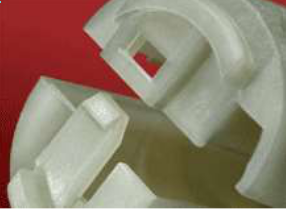
\includegraphics[scale=0.4]{img/cantilever.png}
    \caption{Cantilever Snap}
    \label{snap}
\end{figure}
\indent For controlling, Side Approach strategy is used to assemble the snap parts and Relative Change Based Hirearchical Taxonomy System (RCBHT) is used to sample the force/torque signals of the whole process.
\section{Control Strategy}
The control strategy is fixed. The assembly process contains four state: Approach state, Rotation state, Insertion state, Mating state. In approach state, the upper part approaches to the lower part. After approach state, the upper part rotates until the other two sides of the upper part and the lower part contact. Then force increase to insert the upper part into the lower part. The assembly is finished in Mating state. Details about this can be seen in Appendix.\\
\begin{figure}[h]
    \centering
    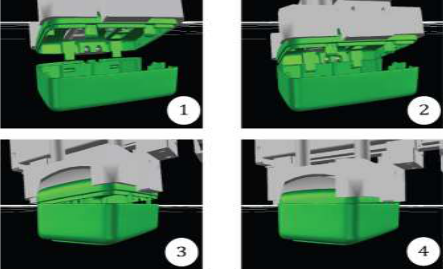
\includegraphics[scale=0.3]{img/controlStrategyFourStep.png}
    \caption{Four control states}
    \label{RCBHT}
\end{figure} 
\section{Relative Change Based Hirearchical Taxonomy System}
The relative change-based hierarchical taxonomy is the state estimation technique that represents the states by hierarchically abstracting snap assembly for force/torque data in increasingly intuitive ways. Five increasingly abstracted layers were used to encode the relative change ub with the force signatures. The taxonomy is consisted by five increasing abstracted layers, including Primitive layer, Motion Composites layer, Low-level Behavior layer, High-level Behavior and Snap Verification Layer. The layers is shown in \\
\begin{figure}[h]
    \centering
    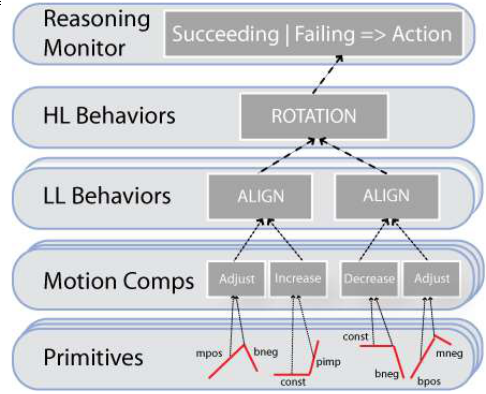
\includegraphics[scale=0.3]{img/fiveLayers.png}
    \caption{Five Layers of RCBHT}
    \label{RCBHT}
\end{figure} 
\indent In our work, we used three lower layers instead the five layers. The details about RCBHT can be seen in \cite{2012IROS-Rojas-RCBHT}. In this section, we will only describe the three lower layers.
\subsection{Primitive layer}
In the primitive layer, each signal is partitioned into linear segments with linear regression with a coefficient. Nine ranges of value of coefficient were labeled by nine different labels. The labels indicate nine ranges of gradients. The upper layers are based on Primitive layer labels.
\subsection{Motion Composites layer}
Motion Composites are consisted of multi-labels of Primitive layer. Two or above similar labels of Primitive layer produced a Motion Composite label. This more abstracted labels attenuate the noise and condense the information.
\subsection{Low-level Behavior leyer}
Being more abstracted, labels of Motion Composite Layer form another layer, Low-level Behavior layer. In this layer, information became more purer and represent the process more intuitively.\\

\indent Details about RCBHT can be seen in appendix.



	% vim:ts=4:sw=4
%
% Copyright (c) 2008-2009 solvethis
% Copyright (c) 2010-2012 Casper Ti. Vector
% Public domain.

\chapter{Classification with SVMs and the RCBHT}
In this section we will introduce a binary classifier using Support Vector Machines and feature inputs from RCBHT labels. The first three layers of the RCBHT taxonomy are of importance to the classification problem. Labels from these three layers are used to construct fixed-length feature vectors. The premise of constructing a feature vector out of RCBHT labels is that success cases have similar patterns in all six axis and similar patterns indicate the similar gradient of each separation of the signal.

\indent The left four signal figures are success cases and right four are failure cases before Rotation state. The success cases are in similar patterns while the failure cases are different from the success cases diversely. With diverse gradients of different patterns, RCBHT can be used in our work.

\indent In \ref{sfsignal}, the four FT figures on the left represent success cases. The four FT figures on the right represent failure cases before the Rotation state. The success cases posses similar patterns while the failure cases are different from the success cases in a number of diverse manners. The difference between success and failure cases is significant enough that a binary set of classes can be extracted to ascertain success from failure.

\begin{figure}[h]
    \centering
    \includegraphics[scale=0.3]{./img/1success.eps}
    \includegraphics[scale=0.3]{./img/1failure.eps}
    \caption{Success Fx signal and Failure Fx signal}
    \label{sfsignal}
\end{figure}

\indent Thus, feature vectors were created by using encoded behavior labels from the RCBHT. Different feature vectors were constructed from different RCBHT layers. Specifically, we used behaviors from the Primitives, Motion Composition, and Low-Level Behavior layers to build three different feature vectors.  . The feature vector constructed from RCBHT label sets have few dimensions, at most 9. A typical feature vector, may include upto 2000 sample points for even a 10-second assembly with a sampling frequency of 200Hz.

\indent This approach assumesthat once the classifier is trained, it can only be used for assemblies with same configuration. If snaps with different geometries, strategies, or sensor positions are used, then the signal patterns would change significantly and the classifier would failAny change of configuration requires retraining of the classifer under that new configuration.

\section{Feature Vector Constructing}
\indent With the RCBHT, we sample the whole assembly using Primitive labels, Motion Composites labels, and Low-level behavior labels. Each axis, $F_{i}$, contains n entries, each represent a label type $e_{j}$. Such that $F_{i} = {e_{1}, e_{2}, \dots , e_{n}}$. The whole vector is consist of six FT axis, $F_{x}, F_{y}, F_{z}, M_{x}, M_{y}, M_{z}$. With respect to labels,The primitive layer yields a set of nine labels independently for each axis , the MC layer in turn yields seven lables, and the LLB also yields seven labels. The feature vector will be conducted containing 6 axis, as $[F_{x}, F_{y}, F_{z}, M_{x}, M_{y}, M_{z}]$. Take the vector representing Primitive layer if in $F_{x}$, bpos occurs twice, mpos occurs once, and the other axis do not have labels (which is an impossible case but just for better understanding), the final vector will be constructed as $[2, 1,\underbrace{0,0, \dots, 0}_\text{52 zeros}]$     \\
\indent A detailed representation of Primitive, Motion Composites, and Low-level behavior sets can be seem in \ref{featureVector}.
\begin {table}[h]
\centering
\caption {Feature Vector Representation}
\label {featureVector}
\begin {tabular}{|llllllllll|}
\hline
Vector Position & 1     & 2     & 3     & 4     & 5     & 6     & 7     & 8     & 9     \\ \hline
Primitive Layer & bpos  & mpos  & spos  & bneg  & mneg  & sneg  & cons  & pimp  & nimp  \\ \hline
MC Layer        & a     & i     & d     & k     & pc    & nc    & c     &       &       \\ \hline
LLB Layer       & FX    & CT    & PS    & PL    & AL    & SH    & U     & N     &       \\ \hline
\end {tabular}
\end {table}

\section{Classify Feature Vector}
After constructing the feature vectors, the classifer should be trained using the success and failure cases. Among different techniques for supervised classification, linear Support Vector Machine was chosen. In this section, we will discuss classifier implementation and review Support Vector Machine and kernel function.\\
\section{Support Vector Machines}
The Support Vector Machine method finds a hyperplane that separate cases with different labels. Predictions are made when all samples, represented by points, are far away from a hyperplane, inidicating that the presented hyphothesis is credible. The hyperplane can be represented as: $\omega^{T}x + b = 0$, where $\omega^{T}$ is the multiplying factor of the hyperplane, and b is the bias from the zero point. Each point, the deviation can be represented as: \\
\begin{equation}
    \hat{\gamma}^{(i)}=y^{(i)}(\omega^{(i)}x+b)
\end{equation}
Here $(y^{(i)}, x^{(i)}$ is a single case where $y^{(i)}$ indicates whether this case succeeded or not. Outcome is represented as  {1, -1} respectively. $x^{(i)}$ is the vector input for training and testing. $\hat{\gamma}^{(i)}$ is the functional margin of this case. To have a nice hyperplane, we need to let as many as possible points to get as far away as well from the hyperplane. That's to say,
\begin{equation}
    \begin{split}
        max\quad&\gamma \nonumber \\
        s.t.\quad&\gamma = \underset{i = 1,\ldots,m}{min}\hat{\gamma}
    \end{split}
\end{equation}
Here $\gamma$ is the geometric margin of points from hyperplane. This equation shows that the nature of SVM is to find a hyperplane to maximize $\gamma$, which is the least functional margin of $\hat{\gamma}$.
\section{Classifier Implementation}
\indent Implementing the SVM classifier takes account the Lagrange duality problem \cite{hager1976lagrange} and the SMO algorithm \cite{keerthi2001improvements}. Many SVM open library existed, among which, libsvm \cite{CC01a} was chosen with Gaussian Kernel \cite{keerthi2003asymptotic}. \\
\begin{description}
    \item[First] \hfill \\
        Firstly, the signal data will constructed into labels of different layers as shown in \ref{fig:hlbehav} \cite{2013IJMA-Rojas-TwrdsSnapSensing} \\
\begin{figure}[h]
    \centering
    \includegraphics[width=4.50in, height=1.75in]{./img/encl2/6.png}
    \caption{This figure shows data related to the first four layers of the RCBHT. (1) The Primitive Layer: red line linear segments try to approximate original data and represent primitives. (2) The Composites Layer: composed by analysis of neighboring primitives. Corresponding labels appear in black at the top-most part of screen. (3) The LLB Layer: LLBs composed by analysis of neighboring composites. Corresponding labels appear in uppercase red letters below the graph. (4) The HLB Layer: HLBs derive from key LLBs. Corresponding labels appear in green at the bottom-most part of screen.}
    \label{fig:hlbehav}
\end{figure}
        Now let's construct the feature vector. Here the labels of MC layer are [d, a, a, a, i, k, a, d, i, a, i, a, k, a, a, k, a, a, i, a, a, a, k, a, k] (The strategy we used only contains 4 states, the example here is expedient for illustration). Then the feature vector will be constructed as [14, 4, 1, 5, 0, 0, 0]. Notice that the data here is only the data of $F_{x}$. Let $F_{x} = [14, 4, 1, 5, 0, 0, 0]$
    \item[Second] \hfill \\
        Repeat the first operation until the other five axis of data are constructed. The overall feature vector is $[F_{x}, F_{y}, F_{z}, M_{x}, M_{y}, M_{z}]$.
    \item[Third] \hfill \\
        Label the feature vector. Here this example case is a success case, so label it with 1 (Failure cases are labeld with -1. Actually they can be labeled as any number as long as it is different from the label of success cases). 
    \item[Forth] \hfill \\
        Repeat the first three steps for all cases. Combine all cases into a matrix of all vectors, and a vector of all labels. Then trained them with SVM and a SVM struct will be returned. This struct recorded the hyperplane and all kinds parameters needed for SVM and prediction of new cases will use this struct. In other words, the training end. The use of libsvm can be seem in \cite{CC01a}.
\end{description}














	\chapter{Experiment Result}
The SVM classifier is trained and tested with a total of 192 assemblies. Among those assemblies, 150 are failure cases with deviation of x, y, and $\phi$ direction, and 42 are success cases. Two scenarios are considered: (i) early failure detection, considering the labels of Approach state and (ii) late failure detection, consisting of labels in all four states of the Assembly task.

\section{Training and Testing Methodology}
Two methods are conducted in training and testing. The 192 assemblies are separated into two groups, for testing and training. (i) For testing, we randomly selected 96 samples (75 failures and 21 success). (ii) For training, we used the remaining 96 samples (Also 75 failures and 21 success). For the first method, named preset training (PT), we started our training from 5 cases (1 success and 4 failures). Then we append samples into our training group. For every 4 failure cases we include 1 success case. For the second method, named random training (RT), we randomly selected the training samples, increasing from 5 to 96 samples but keep the ratio of success samples and failure samples of 1/4.  

We ran the two methods for 100 times respectively. In the following subsections we will describe our findings of the two methods.
\section{Early Failure Detection}
For early failure detection we construct our feature vectors consisting of those labels that show only during the Approach state for all six force/torque axes. With feature vector consisting P labels only, the classifier reacged an average asymptotic maximum value of 93.72\% and a minimum of 89.6\% for method using the RT method. The values for the PT method are 93.67\% and 89.6\% respectively.

\indent The figure left is with the PT method while the right one is with the RT method.
\begin{figure}[h]
    \centering
    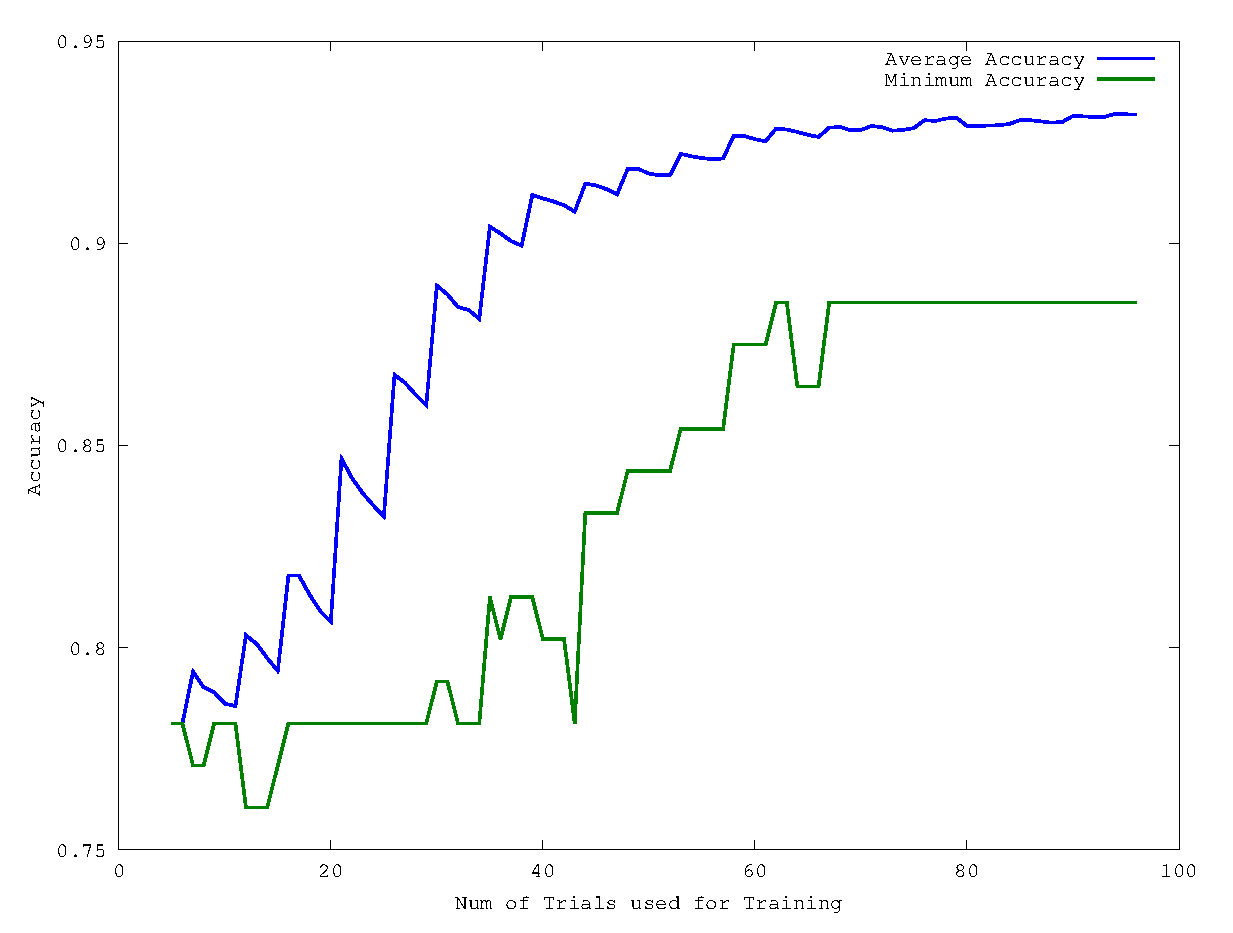
\includegraphics[scale=0.3]{./img/fixTrain/3.eps}
    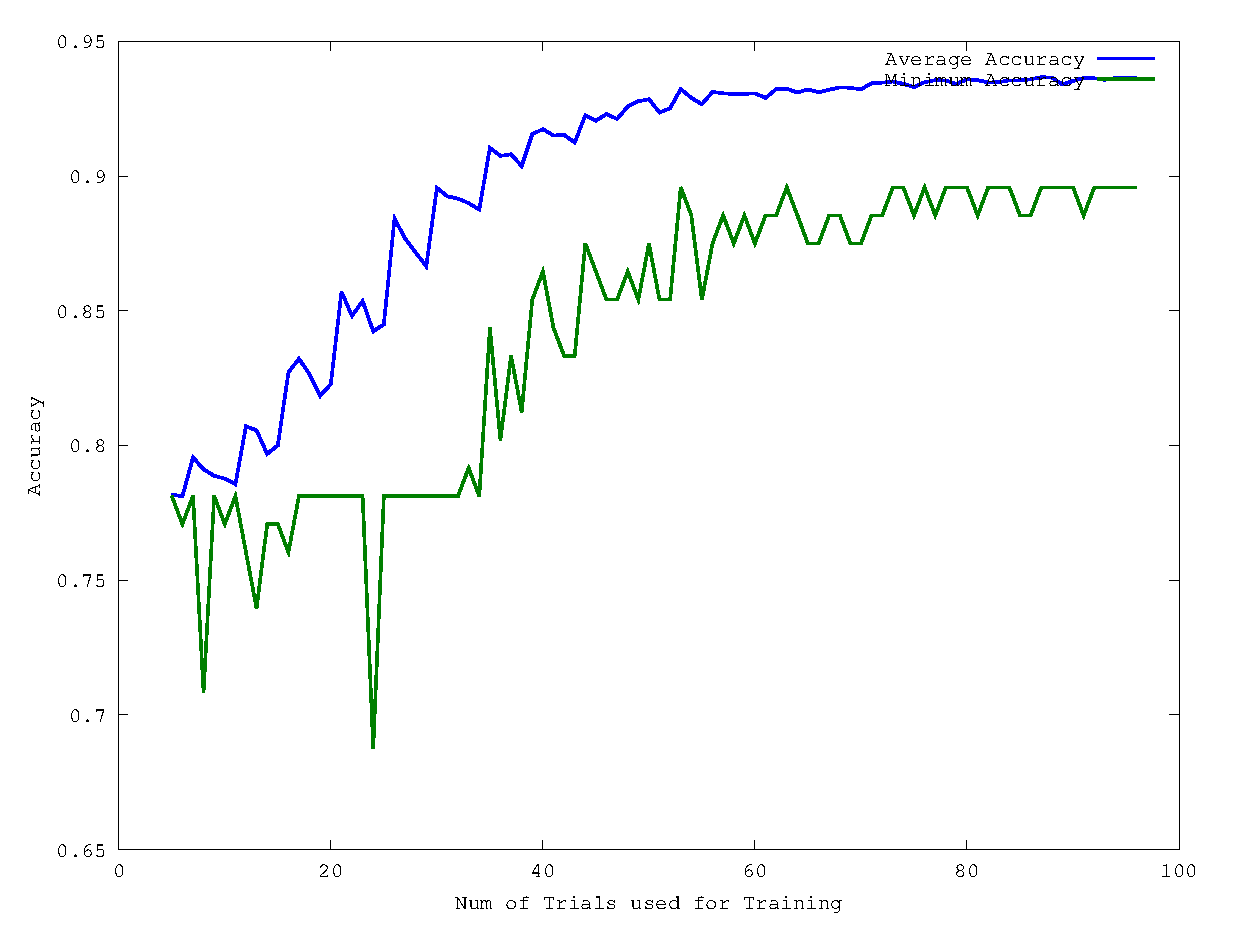
\includegraphics[scale=0.3]{./img/randTrain/3.eps}
    \caption{Classifier with P labels}
    \label{P}
\end{figure}

\section{Late Failure Detection}
For the late failure detection we construct our input feature vector consisting of those labels that show throughout all four states of the task (Approach-Mating) for all six force/torque axes. With feature vector consisting MC and LLB, we conducted the same experiment as it of early failure detection. For the LLB and MC layers, with the PT method, the classifier had an average asymptotic maximum value of 99.59\% and 99.25\% respectively and a minimum of 98.9\% and 93.8\% respectively. The MC classifier reached asymptotic value after about 70 trails while the LLB classifier did so after approximately 22 trials. 

\indent The figure left is with the PT method while the right one is with the RT method.
\begin{figure}[h]
    \centering
    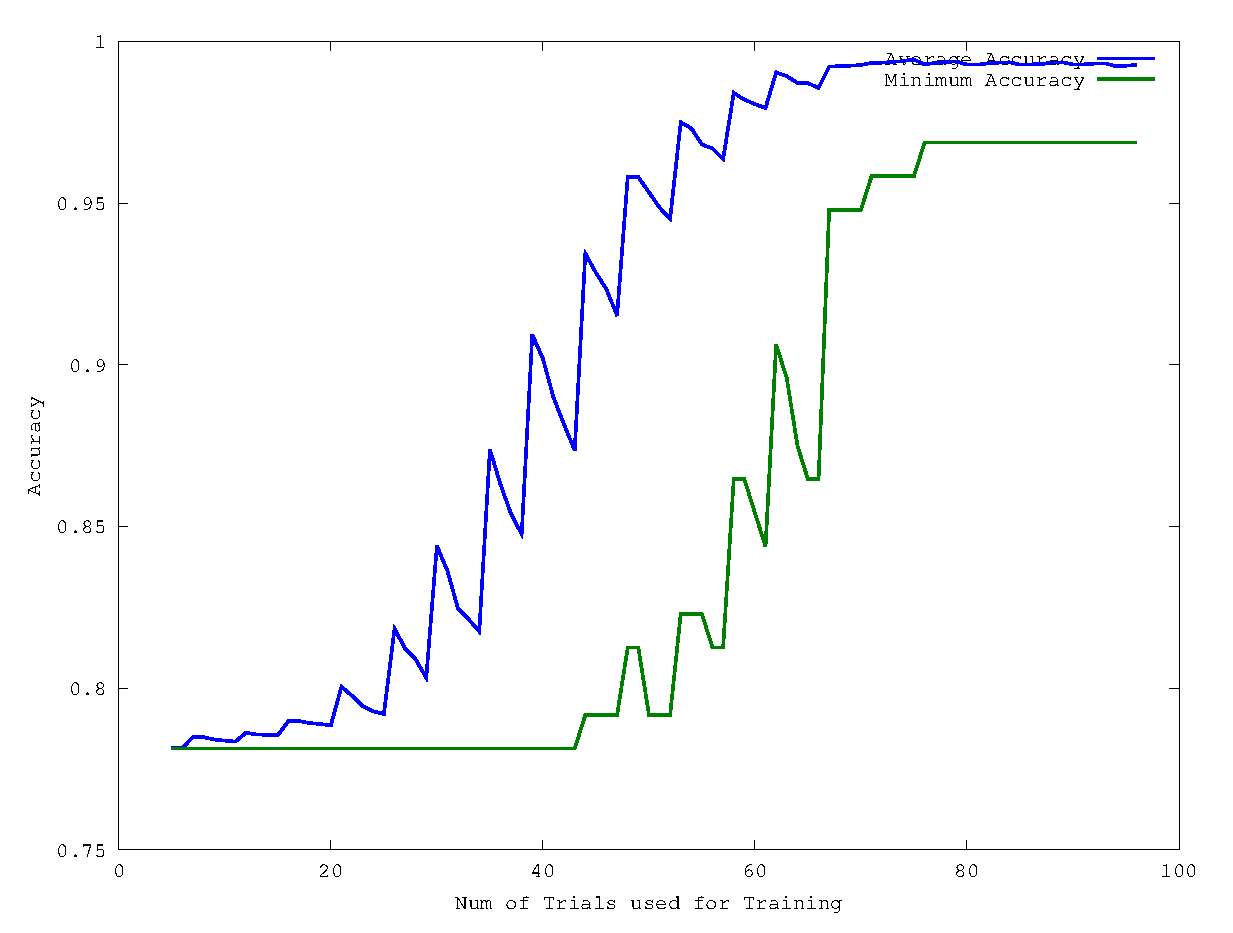
\includegraphics[scale=0.3]{./img/fixTrain/2.eps}
    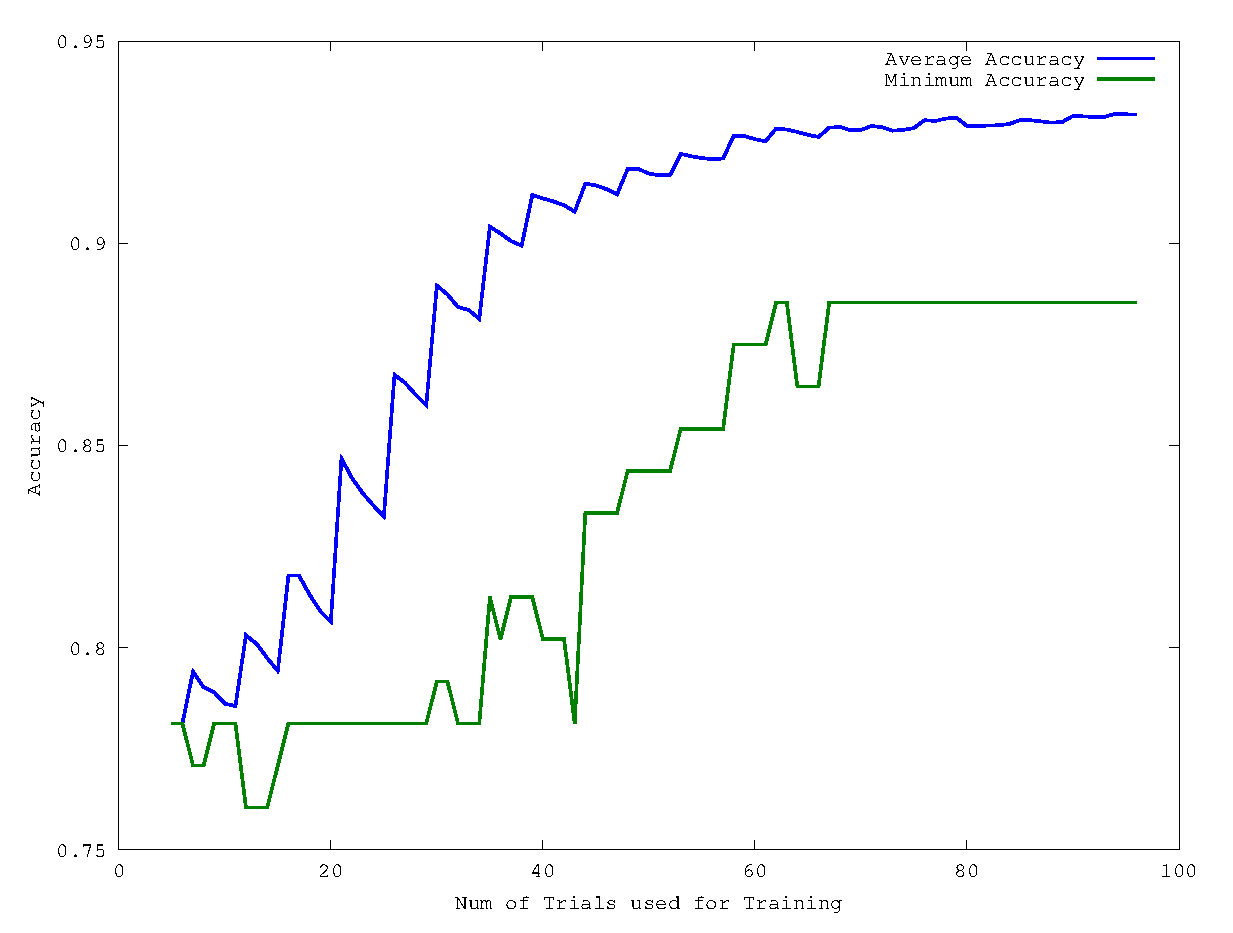
\includegraphics[scale=0.3]{./img/fixTrain/3.eps}
    \caption{Classifier with MC and LLB with the PT method.}
    \label{fixMCLLB}
\end{figure}

\indent With RT method, the result is very much the same as PT method.
\begin{figure}[h]
    \centering
    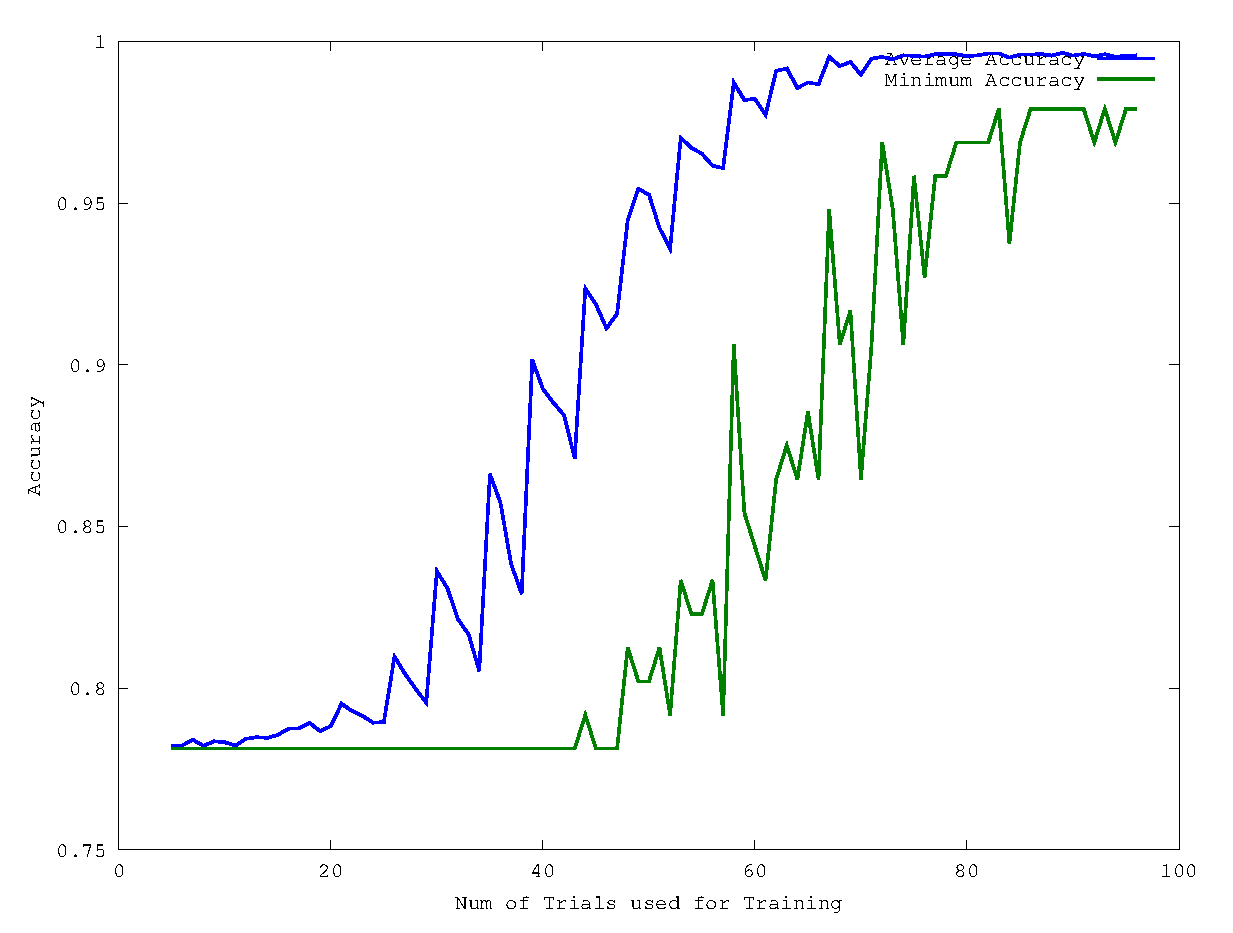
\includegraphics[scale=0.3]{./img/randTrain/2.eps}
    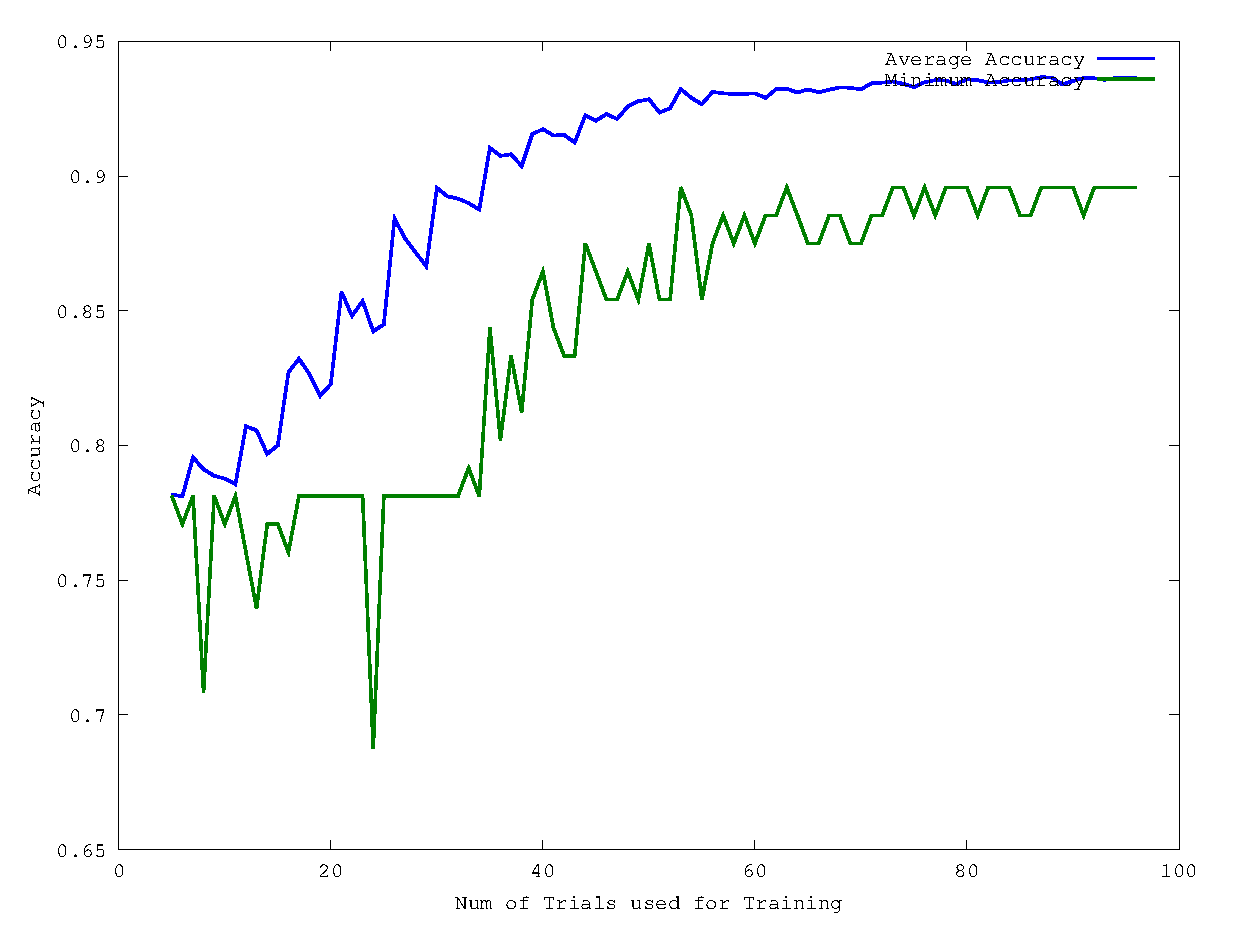
\includegraphics[scale=0.3]{./img/randTrain/3.eps}
    \caption{Classifier with MC and LLB labels with RT method}
    \label{randMCLLB}
\end{figure}

	%\chapter{Conclusion and Future Work}

	\chapter{Discussion and Future Work}
\section{Discussion}
The high accrucy of using the whole process of LLB and MC indicates that there are difference between success cases and failure cases and RCBHT can show it. But when only the Approach stage was measured, there are too little information to identify the failure. In some cases, there was only one LLB, which began at the very start and didn't finished, for some of their axis. While little information caused the lack of diversity, too much information with noise also prevent a good hypothesis. The P of the whole process contain too much noise of viberation and friction. For only the approach stage, though the noise may disturb the prediction accrucy, the Classifier still give good hypothesis. For the whole, the noise is too much. \\
\indent Then we can predict the ongoing case early in the assembly process, the Approach stage. We had more free space in refining the lateral actions. The failure assembly task can be detected and stopped only after the Approach stage to prevent the damage of the machine arm or breaking the cantilever snap. \\ 
\indent The limitation of this approach is that we assume the machine hand got some problems at the begining, or say, the assembly is wrong from the begining. If the machine hand got into problem during the assembly, we could not realized at the very moment.
\section{Future Work}
We should consider these two improvement we could make: (1)Classify the failure cases into subsets and (2) be able to detect failure as soon as it happens. \\ 
\indent Classifying the failure cases with the force/torque signal into subsets, we would have the posterior of the diviation distribution and the corresponding diviation of specific signal. Failure cases with only one or two axis of diviation can be success classified currently but we could not effectively implement it with three axis of diviation. \\
\indent Being able to detect failure at the moment it got away from the right path is necessary because these kinds of robotic problems would cause huge problems. The damage would be acute at the first wrong behavior. If the hypothesis could be made after this behavior occurs, or the second time it began, the machine arm had been have some damage.   

	% 结论。
	%\include{chap/conclusion}

	% 正文中的附录部分。
	\appendix
	% 排版参考文献列表,并使其出现在目录中。
	% 如果同时要使参考文献列表参与章节编号,可将“bibintoc”改为“bibnumbered”。
	\printbibliography[heading = bibintoc]
	% 各附录。
%	% vim:ts=4:sw=4
%
% Copyright (c) 2008-2009 solvethis
% Copyright (c) 2010-2012 Casper Ti. Vector
% Public domain.

\chapter{pkuthss 文档模版的实现}


%	% vim:ts=4:sw=4
%
% Copyright (c) 2008-2009 solvethis
% Copyright (c) 2010-2012 Casper Ti. Vector
% Public domain.

\chapter{The RCBHT}\label{sec:RCBHT}

%--------------------------------------------------------------------------------------------------------------------------------------------------

% Overview

The hierarchical taxonomy's goal was to connect human apropos actions like: ``approaching", ``rotating", ``aligning", ``snapped", and ``mated" with LLB's in a context-sensitive manner. One of the main challenges encountered in interpreting force signals is their inherent noise and spatio-temporal complexity. However, the force signals do inherently possess characteristics that describe the task at hand. The authors hypothesized that such characteristics could be extracted by looking at how temporal relative changes were associated to each other and contextualized by the state in which they occur. In so doing, intuitive behavior sequence's can be extracted and their outcome examined. This level of discrimination is significant as it can be expanded to a real-time implementation and allow to reason about the state to perform corrective motions if necessary.
To bootstrap the approach, we partitioned the data into linear segments that approximate the data and classify the gradients according to magnitude per a small set of criteria. The next layer of abstraction examines at ordered-pair primitive sequences, and according to the gradient patterns presented and a small set of classification criteria, they are categorized into one of several types of motion compositions. The third layer abstracts sequences of motion compositions to identify LLB's, while the fourth layer looks at what LLB's are present in which states to determine if desired high-level behaviors are present. The final layer outputs the verification process results' according to whether or not the desired sequence of HLB's is present or not. A visualization of the hierarchical taxonomy can be seen in Fig. \ref{fig:Taxonomy}.
%--------------------------------------------------------------------------------------------------------------------------------------------------
\begin{figure}[h]
    \centering
    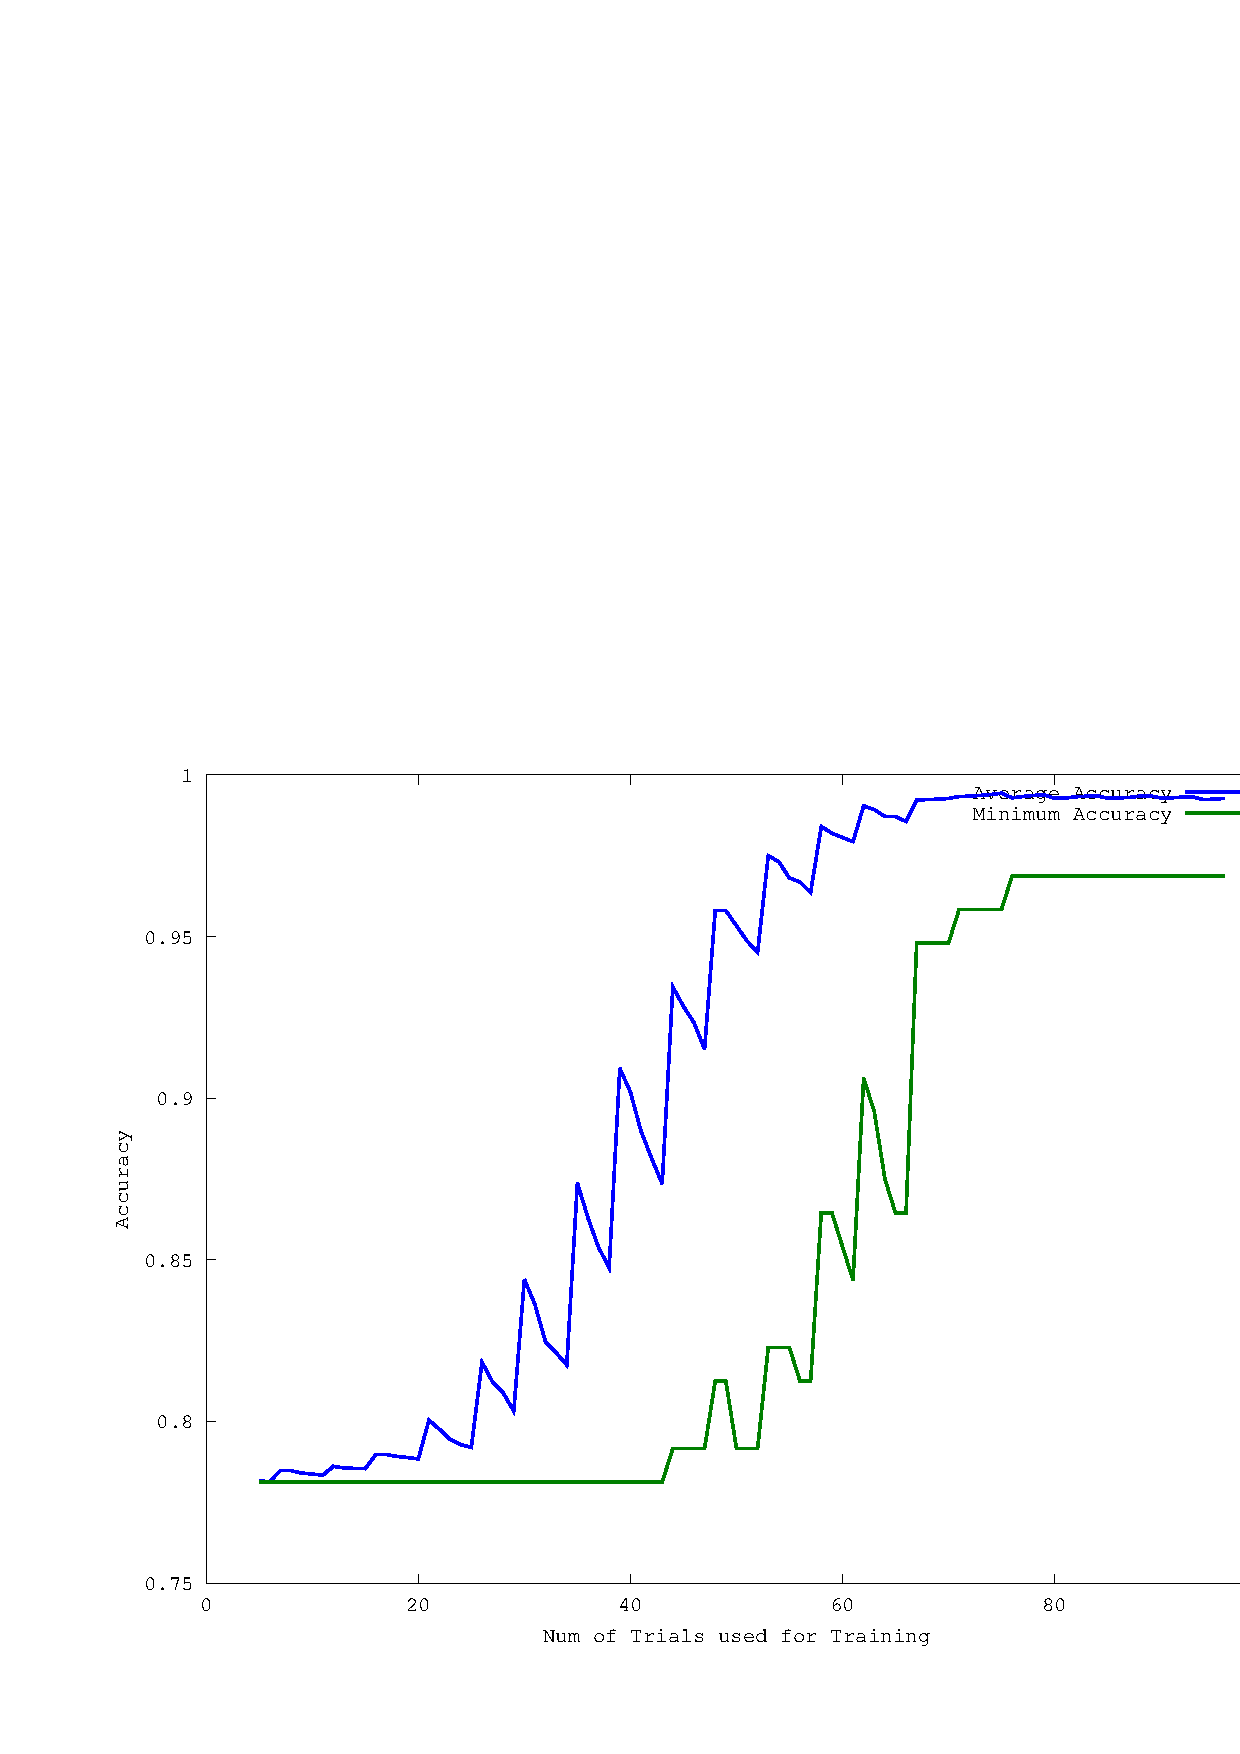
\includegraphics[width=3.35in, height=2.5in]{./img/encl2/2.png}
    \caption{The Relative Change-Based Hierarchical Taxonomy (RCBHT) for Cantilever-Snap Assembly Verification.}
    \label{fig:Taxonomy}
\end{figure}
%--------------------------------------------------------------------------------------------------------------------------------------------------
%--------------------------------------------------------------------------------------------------------------------------------------------------
\section{Primitive Layer} \label{subsec:Primitives}
%--------------------------------------------------------------------------------------------------------------------------------------------------
% Primitives: Signal Approximation through linear fits + Gradient + Data Structure
The primitives layer requires that each signal is partitioned into linear segments of data that closely approximate the original signal. Linear regression in concert with a correlation measure (the determination coefficient $R^2$) is used to partition the data whenever a minimum correlation threshold is crossed. If the determination coefficient drops under a given threshold the linear fit is partitioned and a new regression is started. The $R^2$ coefficient is a correlation measure that studies the ratio of the sum of the squares of the residual errors between the original data $y$ and the fit data $\hat{y}$ to the sum of the variance $\sigma{_y}^2$ as shown in Eqtn. \ref{eqtn:DeterminationCoefficient}.
%--------------------------------------------------------------------------------------------------------------------------------------------------
\begin{equation}
\label{eqtn:DeterminationCoefficient}
    R^2 = 1 - \frac{\sum{(y-\hat{y})^2}}{\sigma{_y}^2}
\end{equation}
%--------------------------------------------------------------------------------------------------------------------------------------------------
The threshold used to partition the data was set at 0.70, such that if the correlation dropped to under $70\%$, a linear segment or ``partition" would be generated, and a new one would start at the next data point. The data was traversed by a window equal to five data points (the data was sampled at a frequency of 1kHz by the simulation). The threshold values and the window length were empirically selected to partition the data sufficiently to capture relevant changes in the signals.
Each partition was accompanied by a data structure with seven types of information about itself: the average value across data points, the maximum value, the minimum value, the start time, the end time, the gradient value, and a gradient label. With respect to the latter, nine gradient labels (positive impulse, `pimp'; big, medium, and small positive gradients, `b/m/spos'; constant gradients, `const'; and their negative equivalents, `nimp', `b/m/s/neg') were assigned according to ranges summarized in Fig. \ref{tbl:GradientRangeValues}.
%--------------------------------------------------------------------------------------------------------------------------------------------------
\begin{figure}[h]
    \centering
    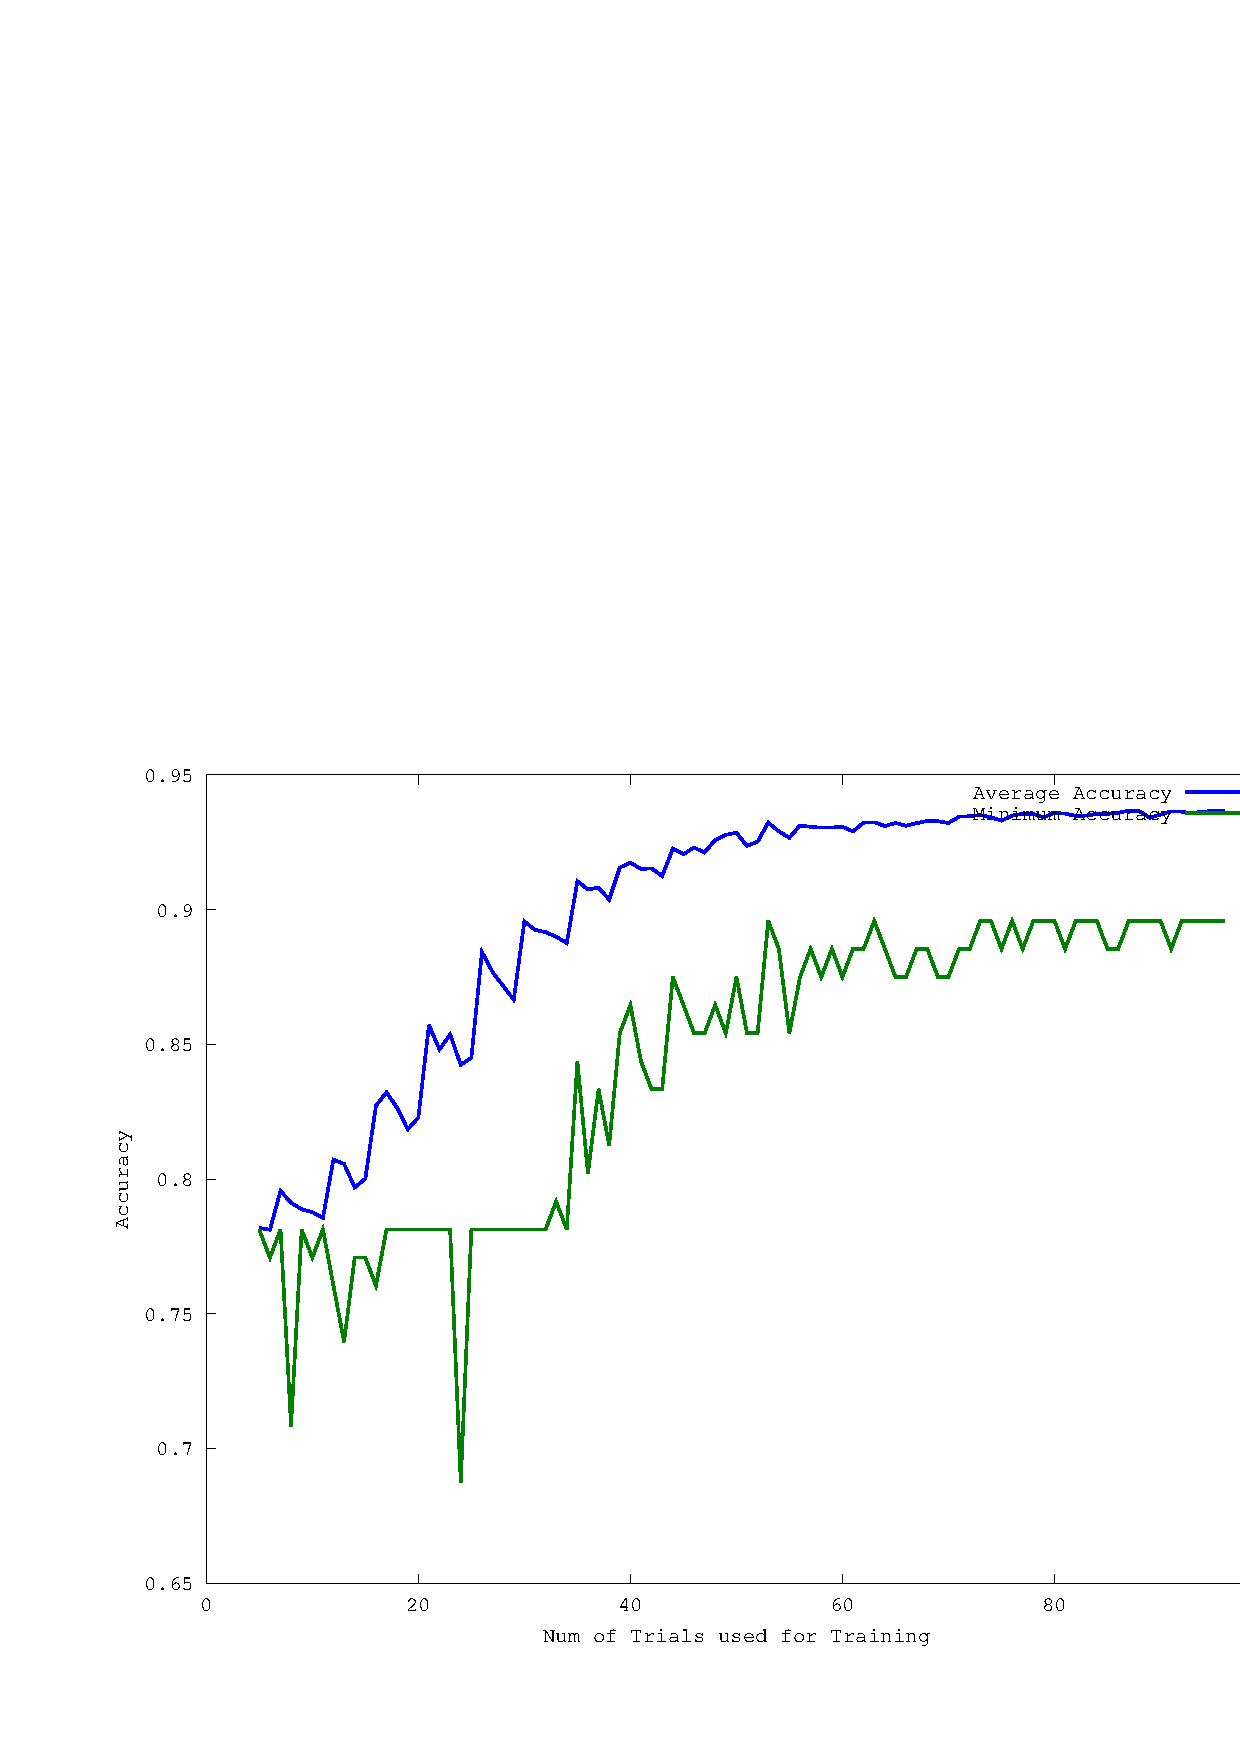
\includegraphics[width=2.75in,height=1.5in]{./img/encl2/3.png}
    \caption{Gradient values classification for the Primitives layers.}
    \label{tbl:GradientRangeValues}
\end{figure}
%--------------------------------------------------------------------------------------------------------------------------------------------------
The classification first attempts to separate instances of data in which contact or mating takes place. On the one hand, contact phenomena is characterized by very rapid and large changes in force signals, almost approximating an impulse. To this end, positive and negative impulses were categorized for gradients with values greater or less than 70. On the other hand, for mating situations, there is little or no change in force, for this reason a constant label was assigned to signals with gradient values less than the absolute value of 1. In between these two extremes we chose to have three gradient categories for both positive and negative signals to give a general idea of the magnitude change registered for a signal. Fig.\ref{fig:hlBehs} shows how the segmentation looks like across all five states (which are represented by five colored boxes) for the force signal in the x direction for PA10 related-experiments.
%--------------------------------------------------------------------------------------------------------------------------------------------------
%\begin{figure}[p!]
%    \centering
%        \includegraphics[width=4.50in, height=1.75in]{../../templates/figures/2012/IROS/PrimitivesFx.eps}
%        \caption{Primitive Layer: each red line represents a primitive that approximates the original signal.}
%        \label{fig:Primitives}
%\end{figure}
%--------------------------------------------------------------------------------------------------------------------------------------------------
%--------------------------------------------------------------------------------------------------------------------------------------------------
\section{Composites} \label{subsec:Composites}
%--------------------------------------------------------------------------------------------------------------------------------------------------
% Composites: Combinations of primitives
The next layer of abstraction identifies seven basic motions compositions (MC) by looking at ordered-pair sequences of primitives. The MC layer set is comprised of: adjustment, increase, decrease, constant, contact, positive contact, negative contact, and unstable motions. The positive and negative contacts, imply the sign of the (gradient) of the action.
A protocol was followed to minimize the effects of noise or erroneous segmentation. With respect to adjustments, primitives with big-to-small positive or negative gradients were considered as a positive or negative primitive category respectively. If a positive grouped primitive was followed by a negative grouped primitive an adjustment classification would be assigned to the ordered pair. Adjustments are motions in which the wrist records a quick `back-and-forth" motion typically seen during alignment or insertion operations as the force controller tries to minimize residual errors. The reason to group positive and negative gradients is to maximize the likelihood of group adjustments even when the rate of change may be slightly different. Furthermore, for this particular category, we used a window of two data points instead of one to look for a matching pair (all other categories looked at the contiguous primitive). That is, if after finding a positive or negative gradient, and if the next data point was not negative or positive respectively, we would look at the next data point to look for a pair. Such procedure mitigates the presence of spurious signals that could prevent the proper grouping of an adjustment movement.
The ordered pair groupings for motion composition classification are summarized in Fig. \ref{fig:MotionCompositions}. Note that the table contains sub-tables representing eight possible motion composition classifications. Each of which can be comprised of different sets of primitive groupings as illustrated in Fig. \ref{fig:MotionCompositions}.
%--------------------------------------------------------------------------------------------------------------------------------------------------
\begin{figure}[h]
    \centering
    \includegraphics[height=1.5in,width=4in]{./img/encl2/4.png}
    \caption{Motion Compositions according to primitive pairs in any order.}
    \label{fig:MotionCompositions}
\end{figure}
%--------------------------------------------------------------------------------------------------------------------------------------------------
As with the primitives layer, 11 pieces of information were collected for each MC: composition label, average value, root means square value, amplitude, the labels of the first and second primitives, the starting and ending times for both primitives, and the average time for both primitives.
%--------------------------------------------------------------------------------------------------------------------------------------------------
\subsection{Refinement} \label{subsubsec:Refinement1}
%--------------------------------------------------------------------------------------------------------------------------------------------------
After the MCs are generated, a refinement phase was used to filter less significant signals and augment more significant signals. To do so, the compositions were analyzed under three contexts: (1) a composition's time duration, (2) a composition's amplitude magnitude, and (3) composition repetition patterns.\\
%--------------------------------------------------------------------------------------------------------------------------------------------------
- Time Duration Context: this filter examines two contiguous MCs. If either composition is seven times bigger than the other, the smaller composition is merged to the larger one and all data is updated correspondingly. The duration ratio was determined empirically.\\
- Amplitude Value Context: this filter pertains to the formation of adjustment signals and constant signals. We considered three possibilities:
(i) If there are contiguous primitives of types PC/NC or NC/PC, and if their amplitude is ten times smaller than the largest amplitude registered in the assembly, then treat them as an adjustment. This criteria seeks to disambiguate real contact signals and false ones by looking at their amplitude. Real contacts are characterized by large values.
(ii) Similarly, if their is either an increase followed by a decrease and vice-versa, and both compositions have a similar amplitude (within ($50\%$) of each other and they have a similar average value ($100\%$) of each other, then merge as an adjustment and update the data correspondingly.
(iii) If there is a sequence of an increase followed by a constant, or a decrease followed by a constant and vice-versa, and they have a similar amplitude ($150\%$)and similar average value ($100\%$), then merge them as a constant and update their information. This last filter targets small noisy signals that appear as increases or decreases but that in effect are constants. The amplitude threshold value is larger here to give more possibilities of catching increases or decreases within the narrow range of the constant's amplitude.
- Repeated Compositions: the last filter takes signals that repeat and merges them as one. This filter is run iteratively until no more repetitions occur in the data.\\
%--------------------------------------------------------------------------------------------------------------------------------------------------
The post-refinement composition layer results are shown in Fig. \ref{fig:hlBehs} for a force signal sample in a Pivot Approach trial.
%--------------------------------------------------------------------------------------------------------------------------------------------------
%\begin{figure}[p!]
%    \centering
%        \includegraphics[width=4.50in, height=1.75in]{../../templates/figures/2012/IROS/CompositesFx.eps}
%        \caption{Composites Layer: motion composites are generated from a sequence of primitives. Their labels are show above the signal.}
%        \label{fig:Composites}
%\end{figure}
%--------------------------------------------------------------------------------------------------------------------------------------------------
%--------------------------------------------------------------------------------------------------------------------------------------------------
\section{Low-Level Behaviors} \label{subsec:llbeh}
%--------------------------------------------------------------------------------------------------------------------------------------------------
% Low-Level Behaviors: Combinations of Composites
The taxonomy's third layer considers motion composition ordered pairs along with signal duration and amplitude to yield classifications. Eight LLB classifications were derived and labeled as: {push, 'PS'}, {pull, 'PS'}, {contact, 'CT'}, {fixed, 'FX'}, {alignment, 'ALIGN'}, {shift, 'SH'}, and {noise, 'N'}. The LLB formulation criteria is similar to those at the MC level. That is, for a pair of increase MCs labels, or decrease MCs labels, or constant MCs labels or adjust MCs labels; pull, push, fixed, or adjust LLBs are assigned respectively. As for contacts, if there is a positive contact followed by a negative one, or vice-versa, a contact LLB is assigned. One major difference between the MC level and the LLB level is introduction a shifting behavior `SH'. Shifts and alignments are similar but differ in that, whenever there are two contiguous adjustment compositions, if the second composite's amplitude is larger than the first, label it as `SH' LLB, if smaller label it `ALGN'.
With regards to the time duration context, if any motion composition lasts more that 100 milliseconds, it can by itself be a low-level behavior, or if the contiguous composition is of the same classification they can also merge correspondingly. If any composition is less than the allotted duration and it does not have a matching pair, it is considered a noisy signal. With regards to the amplitude context, if there are two adjustments within a window of 2 data points, and their amplitudes decrease, render such a pair as an alignment, otherwise consider it a shift (or growing de-alignment). As for paired increase, decreases, and constants, they will yield pull, push, and fixed low-level behaviors correspondingly. Finally, as for contacts, if there is a positive contact followed by a negative one, or vice-versa, or even a stand-alone contact motion primitive, render this is a low-level contact behavior.
%--------------------------------------------------------------------------------------------------------------------------------------------------
\subsection{Refinement} \label{subsubsec:Refinement2}
%--------------------------------------------------------------------------------------------------------------------------------------------------
The LLB layer is also followed by a refinement phase. The latter filters based on the same three contexts as used before:\\
- Time Context: this filter examines two contiguous behaviors (except for contacts). If either behavior is five times bigger than the other, then merge towards the longer behavior and update the data correspondingly. LLB's are longer than compositions, so this threshold value is to be smaller than the one used for the composition's time duration filtering. \\
- Amplitude Context: the amplitude context pertains to alignments and shifts and there are four possible scenarios: (i) If there is a push-pull pair in either order and they have similar amplitudes ($150\%$) and similar average values ($100\%$) render then an alignment. (ii) If there is a shift followed by an alignment, or an alignment followed by a shift, where the second behavior has a smaller amplitude, then merge these as an alignment. This kind of merging is interesting because it can only be seen at this level of abstraction. While there may be a contiguous alignment-shift pair that was irreconcilable earlier, it can now be identified as an alignment. The same is done for a shift. (iii) Finally if there is an alignment followed by a pull or push or viceversa and they have similar amplitude ($50\%$) and similar average value ($100\%$), then merge as an alignment. In this case, after the previous refinement steps have been executed, if there are outstanding alignment-push or -pull pairs, the second behavior is a considered a continuation of the alignment and is merged. Shifts are treated similarly.\\
- Repeated Behaviors: As in the compositions layer, any two repeated behaviors can be merged as one.
The post-refinement LLB layer is shown in Fig. \ref{fig:hlBehs} for a sample signal in the Pivot Approach.
%--------------------------------------------------------------------------------------------------------------------------------------------------
%\begin{figure}[p!]
%    \centering
%        \includegraphics[width=4.50in, height=1.75in]{../../templates/figures/2012/IROS/llBehFx.eps}
%        \caption{LLB Layer: behaviors in this layer are generated from a sequence of motion composites. Their labels are shown below the signal.}
%    \label{fig:llBehs}
%\end{figure}
%--------------------------------------------------------------------------------------------------------------------------------------------------
%--------------------------------------------------------------------------------------------------------------------------------------------------
\section{High-Level Behaviors}\label{subsec:hlbeh}
%--------------------------------------------------------------------------------------------------------------------------------------------------
% High-Level Behaviors: Contextual combinations of low-level behaviors
The fifth layer contextualizes the process monitoring by asking what low-level behaviors principally describe the high-level human apropos behaviors found in the Pivot Approach: Approach, Rotation, (Alignment), Snap Insertion, and Mating\footnote{In actuality, we do not directly assess the Approach stage given that there are no contact forces at this stage. But if the rotation analysis is successful we assume that the approach was too.}.
% Key combinations
Then, if key combinations of LLB's across the six force axes for a specific state are identified, then a certain HLB can be ascertained. For each state and corresponding HLB an LLB or sequence of LLB's are matched with a particular force axis as part of the selected criteria. The criteria is connected both to the PA states, to the Controller Templates, and to the coordinate frame assignments in local coordinates (see Fig. \ref{fig:PA10_ExperimentalSetup} and Fig. \ref{fig:HIRO_ExperimentalSetUp}). Given that we have two implementations of the PA and Controller templates for the PA10-Two Snaps configuration and the HIRO-Four Snaps configuration we have two sets of key LLB criteria. They are presented in Fig. \ref{fig:KeyLLBs}.
%--------------------------------------------------------------------------------------------------------------------------------------------------
%-----------------------------------------------------------------------------------------------------------------------------------------
\begin{figure}[h]
    \centering
%    \subfigure{\label{fig:PA10_KeyLLB}\includegraphics[height=1.25in,width=2.4in]{./img/encl2/4.png}}
%    \hspace{0.04cm}
    \label{fig:HIRO_KeyLLB}\includegraphics[height=1in,width=2.4in]{./img/encl2/5.png}
    \caption{Comparison of the LLBs for both the PA10 and HIRO experimental configurations.}
    \label{fig:KeyLLBs}
\end{figure}
%----------------------------------------------------------------------------------------------------------------------------------------
\subsection{Key LLB's for PA10-Two Snap Experimental Configuration}
%----------------------------------------------------------------------------------------------------------------------------------------
The reasoning behind the selection of LLB's and axis for the Pivot Approach is intuitive. In state 2, the Rotation state, the wrist maintains a constant force along the z-direction, while the force along the y-direction diminishes as the wrist aligns itself with male part. The rotation about the x-axis can be seen through a series of large alignments along the moment's x-direction. For state 3, all axes are aligning in some form. For force elements, there is an alignment in position, for moment elements there is an alignment in orientation. The only exception to this is the moment about the z-direction. A pattern emerges where the moment axis that corresponds to the wrist's direction of motion for the insertion (i.e. the z-axis for the Pivot Approach) experiences little to no change throughout the assembly due to the nature of parts in the assembly task. For state 4, in the insertion state, Rusli studied typical force patterns for manually effected snap assemblies and states that initial resistance is characterizes the insertion until the snap-catch slips behind the undercut in the mating part, at which time an interlock occurs. In other words, one a large increase in force is expected upon contact, followed by a large decrease in force. Hence, we expect to see a contact label followed by an alignment label. Other axis can expect to experience an alignment at this stage. Finally, for the mating state, all signals should present no motion change and thus be classified with a FX behavior.
%----------------------------------------------------------------------------------------------------------------------------------------
\subsection{Key LLB's for HIRO-Four Snap Experimental Configuration}
%----------------------------------------------------------------------------------------------------------------------------------------
In this experimental configuration, the Rotation controller is applying a constant force in both the x- and z-directions and a constant moment in the y-direction. For this reason we expect to find FX LLB tags in this state. Then, as for the insertion stage, experimental results consistently show that for successful assemblies there are CT LLB tags both in the force's x-direction and in the moment's y-direction. Both are correlated in that they represent the robot's downwards assembly motion. The rest of the axes are either aligning or fixed, that is, ALGN or FX tags should be seen in them. Finally, for the Mating state, there should be no movement and hence no change in gradient values if the structure is stable. FX labels are expected in all axis.
The fourth layer results are shown in Fig. \ref{fig:hlBehs}. If the high-level behaviors can be ascertained, they print on the plot in green color. If they cannot be verified, they plot in red color representing failure.
%--------------------------------------------------------------------------------------------------------------------------------------------------
\begin{figure}[h]
    \centering
    \includegraphics[width=4.50in, height=1.75in]{./img/encl2/6.png}
    \caption{This figure shows data related to the first four layers of the RCBHT. (1) The Primitive Layer: red line linear segments try to approximate original data and represent primitives. (2) The Composites Layer: composed by analysis of neighboring primitives. Corresponding labels appear in black at the top-most part of screen. (3) The LLB Layer: LLBs composed by analysis of neighboring composites. Corresponding labels appear in uppercase red letters below the graph. (4) The HLB Layer: HLBs derive from key LLBs. Corresponding labels appear in green at the bottom-most part of screen.}
    \label{fig:hlBehs}
\end{figure}
%--------------------------------------------------------------------------------------------------------------------------------------------------
%--------------------------------------------------------------------------------------------------------------------------------------------------


	% 以下为正文之后的部分。
	\backmatter

	% 致谢。
%	% vim:ts=4:sw=4
%
% Copyright (c) 2008-2009 solvethis
% Copyright (c) 2010-2012 Casper Ti. Vector
% Public domain.

\chapter{致谢}

感谢Dr. Juan Rojas在本论文写作提供的大力支持。没有他的支持,我没法完成这篇论文。
感谢zhibo的中山latex模板,没有这个模板,本论文写作不会这么顺利。


	% 原创性声明和使用授权说明。
%	\include{chap/originauth}
	% 原创性声明和使用授权说明,不显示页码。
	%\pagestyle{empty}
	%\include{chap/originauth}
	%--成绩评定表--
	% \includepdf[pages=1-2]{chap/grade.pdf}
\end{document}

